\begin{figure}[htbp]
\centering
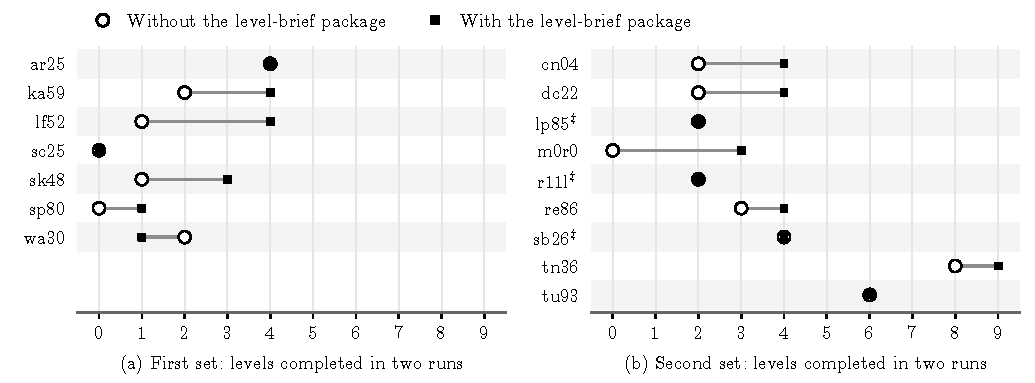
\includegraphics[width=\linewidth]{figures/brief_tests.pdf}
\caption{\textbf{The level-brief package completed more levels in both test sets and completed fewer in one game of the first.} Each row is a game. The horizontal position is the number of levels completed in two runs of up to 100 new actions each. Open circles are the runs without the package, which kept the other memory layers and the object ledger. Filled squares are the runs with it. (a) In the first set, the package was ahead in four games, behind in one (\texttt{wa30}), and level in two, with 17 levels against 10. (b) In the second set, the package was ahead in five games, behind in none, and level in four, with 38 levels against 29. A double dagger marks a game that every run won, so the counts could not differ. Each point sums two runs, and the figure draws no interval.}\label{fig:brief-tests}
\end{figure}
